% Options for packages loaded elsewhere
\PassOptionsToPackage{unicode}{hyperref}
\PassOptionsToPackage{hyphens}{url}
%
\documentclass[
]{article}
\usepackage{amsmath,amssymb}
\usepackage{iftex}
\ifPDFTeX
  \usepackage[T1]{fontenc}
  \usepackage[utf8]{inputenc}
  \usepackage{textcomp} % provide euro and other symbols
\else % if luatex or xetex
  \usepackage{unicode-math} % this also loads fontspec
  \defaultfontfeatures{Scale=MatchLowercase}
  \defaultfontfeatures[\rmfamily]{Ligatures=TeX,Scale=1}
\fi
\usepackage{lmodern}
\ifPDFTeX\else
  % xetex/luatex font selection
\fi
% Use upquote if available, for straight quotes in verbatim environments
\IfFileExists{upquote.sty}{\usepackage{upquote}}{}
\IfFileExists{microtype.sty}{% use microtype if available
  \usepackage[]{microtype}
  \UseMicrotypeSet[protrusion]{basicmath} % disable protrusion for tt fonts
}{}
\makeatletter
\@ifundefined{KOMAClassName}{% if non-KOMA class
  \IfFileExists{parskip.sty}{%
    \usepackage{parskip}
  }{% else
    \setlength{\parindent}{0pt}
    \setlength{\parskip}{6pt plus 2pt minus 1pt}}
}{% if KOMA class
  \KOMAoptions{parskip=half}}
\makeatother
\usepackage{xcolor}
\usepackage[margin=1in]{geometry}
\usepackage{longtable,booktabs,array}
\usepackage{calc} % for calculating minipage widths
% Correct order of tables after \paragraph or \subparagraph
\usepackage{etoolbox}
\makeatletter
\patchcmd\longtable{\par}{\if@noskipsec\mbox{}\fi\par}{}{}
\makeatother
% Allow footnotes in longtable head/foot
\IfFileExists{footnotehyper.sty}{\usepackage{footnotehyper}}{\usepackage{footnote}}
\makesavenoteenv{longtable}
\usepackage{graphicx}
\makeatletter
\def\maxwidth{\ifdim\Gin@nat@width>\linewidth\linewidth\else\Gin@nat@width\fi}
\def\maxheight{\ifdim\Gin@nat@height>\textheight\textheight\else\Gin@nat@height\fi}
\makeatother
% Scale images if necessary, so that they will not overflow the page
% margins by default, and it is still possible to overwrite the defaults
% using explicit options in \includegraphics[width, height, ...]{}
\setkeys{Gin}{width=\maxwidth,height=\maxheight,keepaspectratio}
% Set default figure placement to htbp
\makeatletter
\def\fps@figure{htbp}
\makeatother
\setlength{\emergencystretch}{3em} % prevent overfull lines
\providecommand{\tightlist}{%
  \setlength{\itemsep}{0pt}\setlength{\parskip}{0pt}}
\setcounter{secnumdepth}{5}
\usepackage{booktabs}
\usepackage{caption}
\usepackage{longtable}
\usepackage{colortbl}
\usepackage{array}
\ifLuaTeX
  \usepackage{selnolig}  % disable illegal ligatures
\fi
\IfFileExists{bookmark.sty}{\usepackage{bookmark}}{\usepackage{hyperref}}
\IfFileExists{xurl.sty}{\usepackage{xurl}}{} % add URL line breaks if available
\urlstyle{same}
\hypersetup{
  pdftitle={Detecting Spam},
  pdfauthor={Written by: Daniel Jouran, Ryan Smith, Morgan Wood, \& Shiyunyang Zhao; For STOR 565 Final Project},
  hidelinks,
  pdfcreator={LaTeX via pandoc}}

\title{Detecting Spam}
\author{Written by: Daniel Jouran, Ryan Smith, Morgan Wood, \& Shiyunyang Zhao \and For STOR 565 Final Project}
\date{06 December, 2023}

\begin{document}
\maketitle

{
\setcounter{tocdepth}{2}
\tableofcontents
}
\hypertarget{summary}{%
\section*{Summary}\label{summary}}
\addcontentsline{toc}{section}{Summary}

This report compares the performance of various classification methods for detecting spam emails. Using data provided by the TidyTuesday project on the relative frequency of six different words or characters, we

\begin{enumerate}
\def\labelenumi{\arabic{enumi}.}
\item
  provide predictive models that classify emails as either spam or non-spam with over 85\% accuracy while only using six descriptive statistics of each email,
\item
  provide evidence that tree-based methods outperform many other machine learning models in prediction accuracy, and
\item
  provide insight into the importance of various email statistics in classification. \n
\end{enumerate}

\textbf{Statement on the use of AI tools}

Our group did not use any AI tools during the creation of this report. This includes all categories listed in the ``Project-23-updated.pdf'' file. \n

\textbf{Statement on Member Contribution}

All group members contributed equally to the creation of this report. We will each fill out the Peer Evaluation Survey. \n

\hypertarget{overview}{%
\section{Overview}\label{overview}}

Within this report we aim to provide evidence that the classification of spam emails is possible with very few statistics on each email. To do this, we compare the performance of various machine learning models. Within this report we consider the following models,

\begin{itemize}
\item
  Naïve Bayes,
\item
  Logistic Regression,
\item
  Linear and Quadratic Determinate Analysis (LDA \& QDA),
\item
  K-Nearest Neighbors (KNN),
\item
  Linear and Non-Linear Support Vector Machines (SVM), and
\item
  Multiple Tree-Based Methods.
\end{itemize}

Regarding to the above machine learning algorithms, Naïve Bayes and Logistic Regression allowed us for efficient handling of large datasets and provided clear interpretability. LDA \& QDA helped us understand the complex patterns in emails. KNN was used for its simplicity in similarity-based classification. SVMs adeptly managed the high-dimensional nature of text data. Finally, tree-based methods offered deep insights into intricate feature interactions.

To classify emails as either spam or non-spam, we consider a dataset provided by the TidyTuesday Project\footnote{\url{https://github.com/rfordatascience/tidytuesday/tree/979c7204bb80fd3a00ca1b622de7ebd0f49766bf/data/2023/2023-08-15}}. We will refer to this dataset as the Spam Dataset for the remainder of this report. The Spam Dataset contains the classification of 4601 emails as either spam or non-spam, and provides information on each email in the form of 6 variables which describe the relative frequency of certain words or characters. We describe these variables in detail Section \ref{sec:variables}. Of the 4601 emails, 1813 are spam observations and 2788 are non-spam observations resulting in an approximately 40:60 split.

The Spam Dataset is a subset of the Spam E-mail Database\footnote{\url{https://search.r-project.org/CRAN/refmans/kernlab/html/spam.html}} distributed by R and collected by Hewlett-Packard Labs. In contrast to the Spam Dataset, the Spam E-mail Database contains 57 variables on the same 4601 emails. The Spam Dataset uses 6 variables on the total frequency of various words and characters along with 2 variables related to word and character length from the Spam E-mail Database to instead only display 6 variables on relative frequency.

To compare the performance of each model, our dataset is split approximately 1:1 into a training and test dataset. Each model is trained on 2300 observations, and then performance on the classification of the remaining 2301 test observations is reported.

Our code can be found at the end of this document.

\hypertarget{variables}{%
\section{\texorpdfstring{Variables \label{sec:variables}}{Variables }}\label{variables}}

Perhaps explain each variable and then some basic exploratory analysis.

\hypertarget{logistic-regression}{%
\section{Logistic Regression}\label{logistic-regression}}

\hypertarget{nauxefve-bayes}{%
\section{Naïve Bayes}\label{nauxefve-bayes}}

\hypertarget{tree-based-methods}{%
\section{Tree-Based Methods}\label{tree-based-methods}}

We now consider the predictive performance of tree-based methods. The following section will look at

\begin{itemize}
\item
  Classification Trees,
\item
  Boosting Trees,
\item
  Bagging Trees, and
\item
  Random Forest Models.
\end{itemize}

The models are presented in increasing prediction performance.

\emph{Classification Trees} We begin by training a pruned classification tree as displayed in Figure @ref(pruned\_tree\_plot) where `y' stands for a spam classification and `n' stands for a non-spam classification. We find that the variables corresponding to the length of all-capital strings, the frequency of the exclamation mark ``!'', and the frequency of the dollar symbol ``\$'' are important classifiers, with the frequency of the dollar symbol being the most important. Just as intuition would suggest, for each of these variables, larger values suggest that an email should be classified as spam.

\begin{figure}
\centering
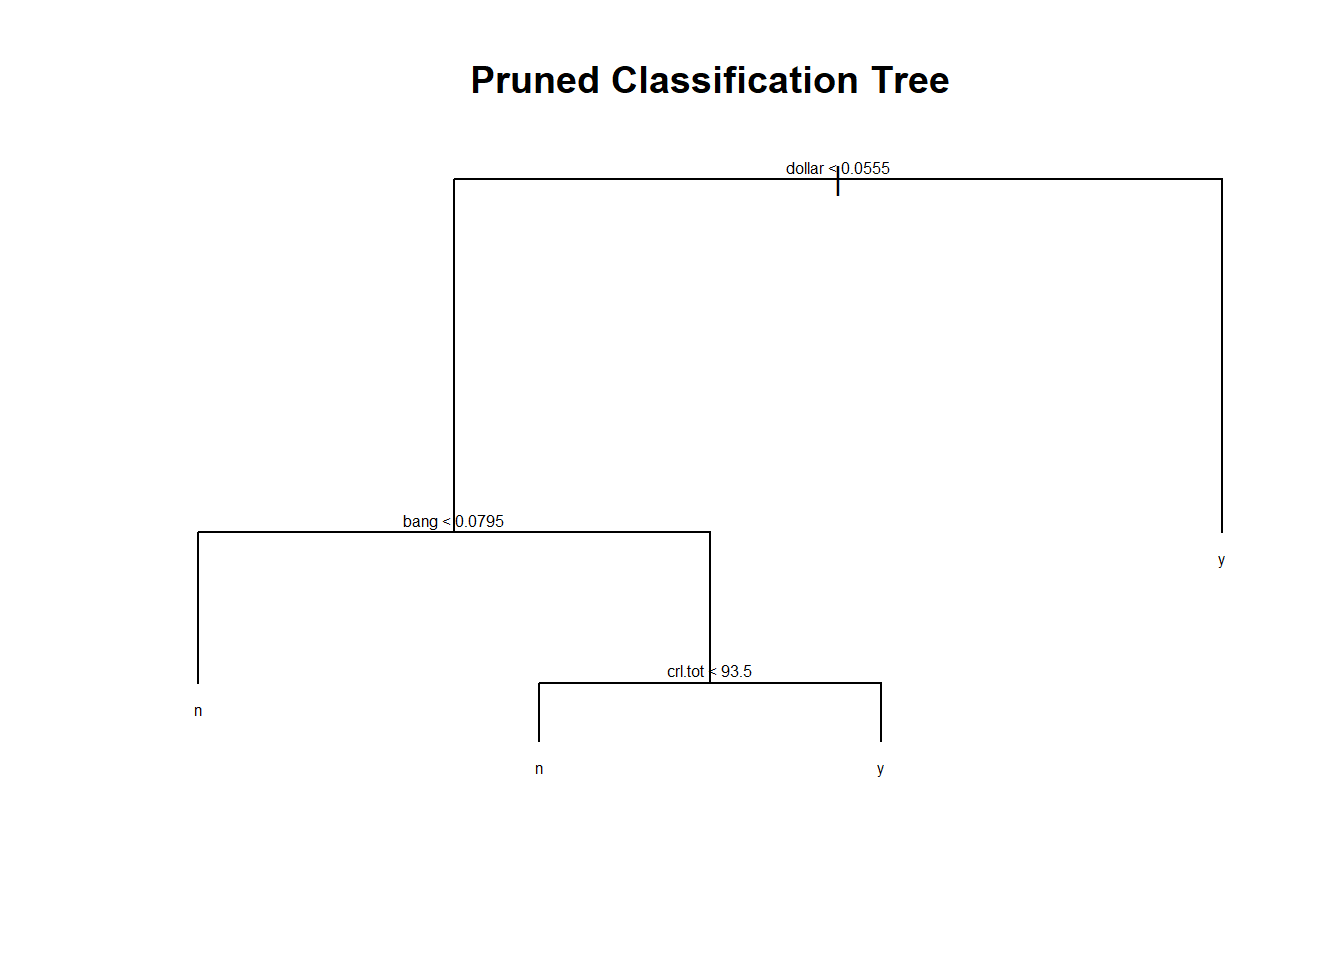
\includegraphics{morgan-figuring-out-references_files/figure-latex/pruned_tree_plot-1.pdf}
\caption{(\#fig:pruned\_tree\_plot)Pruned classification tree which}
\end{figure}

\textbf{Figure 1.}\label{fig:classtree} Pruned classification tree which uses the variables corresponding to the length of all-capital strings, the frequency of the exclamation mark ``!'', and the frequency of the dollar symbol ``\$''. Here `y' stands for classifying an email as spam and `n' stands for classifying an email as non-spam.

\n

For the classification tree displayed above, the tree was grown using deviance and then pruned using misclassification. The performance of the classification tree in Figure \ref{fig:classtree} is summarized in Table \ref{table:classtree}. In total, 84.2\% of the test observations were correctly classified. Of the spam observations, 74.7\% were correctly classified as spam. Of the non-spam observations, 90.4\% were correctly classified as non-spam.

It is worth pointing out that the accuracy of this model is near 85\% while also being interpretable and, arguably, very simple.

\begin{longtable}{l|rr}
\toprule
\multicolumn{1}{l}{} & Truth\_nonspam & Truth\_spam \\ 
\midrule\addlinespace[2.5pt]
Classified\_nonspam & 1264 & 229 \\ 
Classified\_spam & 134 & 674 \\ 
\bottomrule
\end{longtable}

\textbf{Table 1.}\label{table:classtree} Contingency table displaying the predicted verses true classification of emails in the test set using the pruned classification tree in Figure 1.

\n

\end{document}
